\documentclass[tikz,border=6pt]{standalone}
\usepackage{pgfplots}
\pgfplotsset{compat=1.18}
\usepgfplotslibrary{fillbetween}
\usetikzlibrary{arrows.meta}
\usepackage[scaled]{helvet}
\renewcommand{\familydefault}{\sfdefault}
\usepackage[T1]{fontenc}
\definecolor{bordblue}{HTML}{3B82F6}
\definecolor{bordorange}{HTML}{D97706}
\definecolor{navy}{HTML}{1E3A5F}
\definecolor{midgray}{HTML}{8A8A8A}
\definecolor{anncolor}{HTML}{6B7280}
\begin{document}
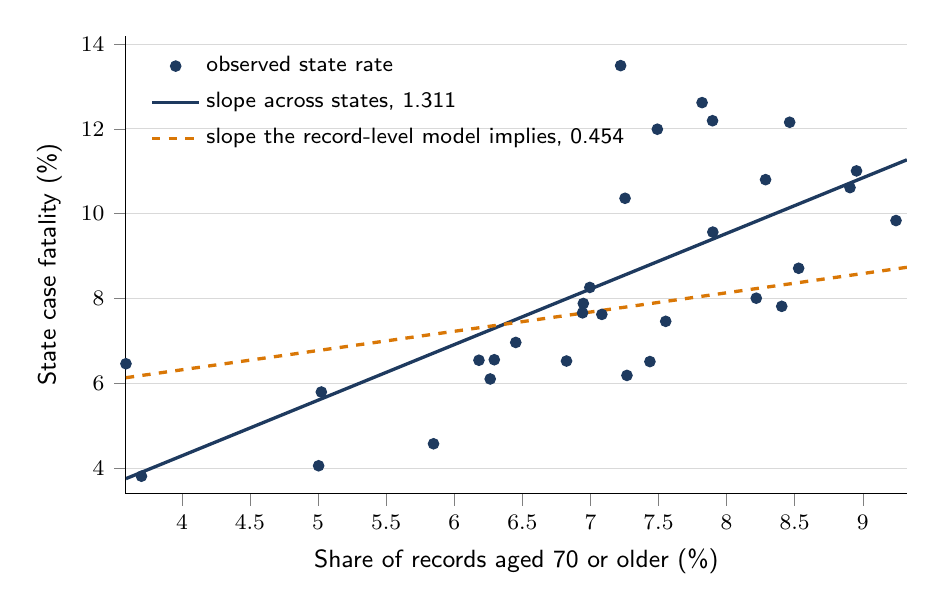
\begin{tikzpicture}
\begin{axis}[width=11.5cm, height=7.4cm,
  xlabel={Share of records aged 70 or older (\%)},
  ylabel={State case fatality (\%)},
  xmin=3.589, xmax=9.324, ymin=3.4, ymax=14.2,
  axis lines=left, axis line style={-}, tick align=outside,
  ymajorgrids=true, grid style={gray!30, line width=0.3pt},
  xlabel style={font=\small}, ylabel style={font=\small},
  tick label style={font=\footnotesize},
  legend style={at={(0.02,0.98)}, anchor=north west, draw=none,
                fill=none, font=\footnotesize, row sep=2pt},
  legend cell align=left,]
\addplot[only marks, mark=*, mark size=1.9pt, color=navy] coordinates {(6.9479,7.8838) (7.4914,11.9919) (3.7031,3.8124) (6.9956,8.2621) (7.0839,7.6267) (6.1814,6.5455) (7.8989,9.5665) (8.2861,10.8027) (5.8478,4.5763) (6.2641,6.1042) (6.8244,6.5273) (8.2178,8.0086) (7.8199,12.6186) (8.9061,10.6150) (7.2218,13.4909) (8.9540,11.0088) (9.2439,9.8383) (8.5290,8.7136) (6.2941,6.5575) (7.4369,6.5143) (7.8967,12.1920) (5.0241,5.7968) (3.5893,6.4630) (7.2682,6.1880) (9.3245,11.9637) (7.5529,7.4627) (5.0040,4.0582) (6.4518,6.9652) (7.2542,10.3636) (8.4631,12.1560) (6.9422,7.6629) (8.4049,7.8164)};
\addlegendentry{observed state rate}
\addplot[navy, line width=1.2pt] coordinates {(3.589,3.7544) (9.324,11.2705)};
\addlegendentry{slope across states, 1.311}
\addplot[bordorange, line width=1.2pt, dashed] coordinates {(3.589,6.1344) (9.324,8.7367)};
\addlegendentry{slope the record-level model implies, 0.454}
\end{axis}
\end{tikzpicture}
\end{document}
